%\documentclass{article}
\documentclass{standalone}
\standaloneconfig{border=2mm 2mm 2mm 2mm}
%\usepackage{geometry}
\usepackage{pgfplots}
\pgfplotsset{width=15cm, height=5cm,compat=1.9}
%\pgfplotsset{compat=1.9}

% We will externalize the figures
%\usepgfplotslibrary{external}
%\tikzexternalize

\begin{document}
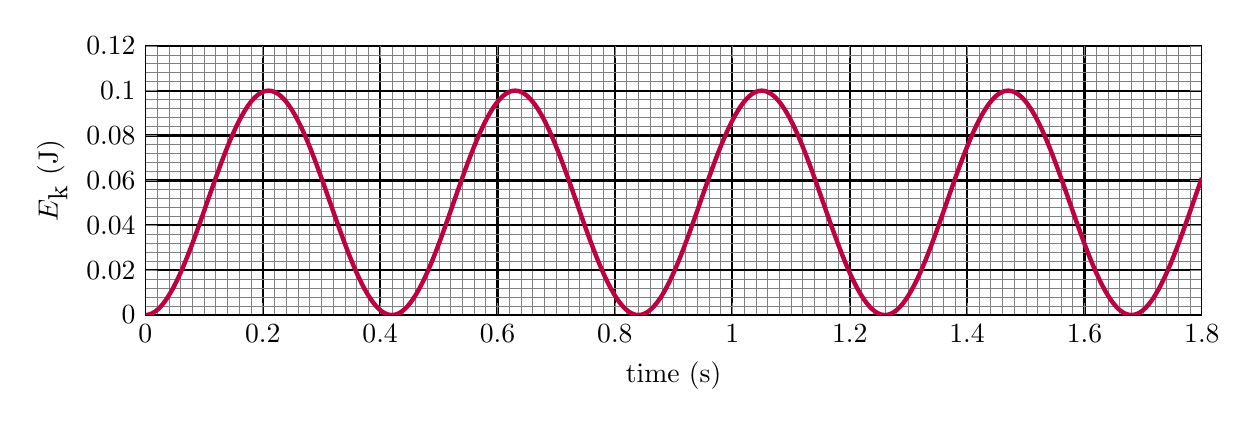
\begin{tikzpicture}
\begin{axis}[
  %axis lines = left,
  xlabel ={time (s)},
  ylabel ={\(E_\textrm{k}\) (J)}, 
  xmin=0.0, xmax=1.8,
  ymin=0.0, ymax=0.12,
  xtick={0.0,0.2,...,1.8},
  ytick={0.0,0.02,...,0.12},
  xmajorgrids=true, ymajorgrids=true,
  minor grid style = {very thin, gray},
  major grid style={solid, thick, black},
  xminorgrids=true, yminorgrids=true, minor tick num = 1,
  %grid style = dashed,
  minor x tick num = 9,
  minor y tick num = 4,
  %minor tick style = {thin, gray},
  %major tick style = {thick, black},
  minor tick style={draw=none},
  xticklabel style={/pgf/number format/.cd, fixed relative, precision=4, /tikz/.cd},
  yticklabel style={/pgf/number format/.cd,fixed relative,precision=3}]
  %style="yticklabel style={
  %/pgf/number format/precision=5,
  %/pgf/number format/fixed}",
  %scaled y ticks=false]

%\addplot[color=red]{exp(x)};
%\addplot[color=blue, samples=100]{x^2};

\addplot[color=purple, domain=0.0:1.8, samples=1000, style=ultra thick]{0.1*(sin(deg(x*3.14159/0.42))^2};


\end{axis}
\end{tikzpicture}
\end{document}